\chapter{Progettazione delle interfacce}
Esistono solo due tipi di design, riuscito e fallito; buono e cattivo (D. Norman).

Il problema è che il buon design non è universale. Un progetto, prodotto o sistema apprezzato da tutti non esiste perché l'esperienza di interazione è soggettiva e quindi dipende più dalla persona che non dall'artefatto e di conseguenza è statisticamente impossibile progettare qualcosa che sia apprezzato da chiunque.

Nel corso vedremo come classificare gli utenti in gruppi e categorie così da poter identificare degli archetipi di persona per i quali andare a progettare l'interazione nella speranza di ottenere dei prodotti che almeno da alcune persone selezionate vengano apprezzati.

Questo perché è bene ricordare che non è possibile progettare l'esperienza di un utente ma si può lavorare per progettare un prodotto che guidi l'utente verso una particolare esperienza da noi identificata come ottimale.

Ci sono due proprietà che sono fondamentali per qualsiasi progetto destinato ad essere utilizzato da persone: Discoverability (rilevabilità) e Understanding (comprensibilità)

\textbf{Discoverability:} è la capacità di un sistema di veicolare e comunicare i propri possibili usi all'utente. Un sistema che a prima vista fa capire all'utente a cosa serve e che cosa ci si può fare ha una buona discoverability. Per avere una buona discoverability si usa tipicamente la \textbf{visibilità}. Se le funzioni dell'oggetto sono visivamente eclatanti è probabile che l'oggetto abbia una buona discoverability.

Un rubinetto con i pomelli ha una discoverability migliore di un rubinetto automatico perché le sue funzioni sono più facilmente identificabili grazie a una maggiore visibilità dei controlli.


\begin{figure}[!h]
	\centering
	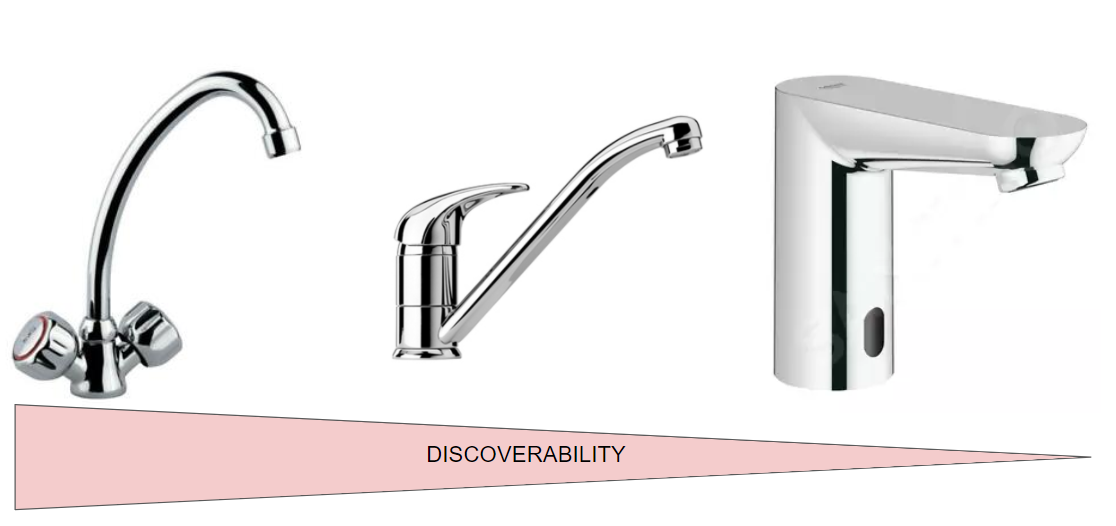
\includegraphics[width=\textwidth]{immagini/discoverability.png}
	\caption{Discoverability and visibility.}
\end{figure}


\textbf{Understanding}: è invece la capacità del prodotto di farsi usare correttamente dall'utente. Se la discoverability è la misura di quanto bene si capisce \textbf{cosa} si può fare con il prodotto, l'understanding invece è la proprietà associata a quanto bene un prodotto dice \textbf{come} si usano le funzioni disponibili.

Per capire come si usa un prodotto non basta infatti aver identificato quali sono i controlli, è necessario dare con facilità risposta alle seguenti domande:

\begin{itemize}
    \item Come si usa il prodotto?
    \item Che funzione ha ciascun controllo?
    \item Come si combinano i controlli?
    \item...
\end{itemize}




\begin{figure}[!h]
	\centering
	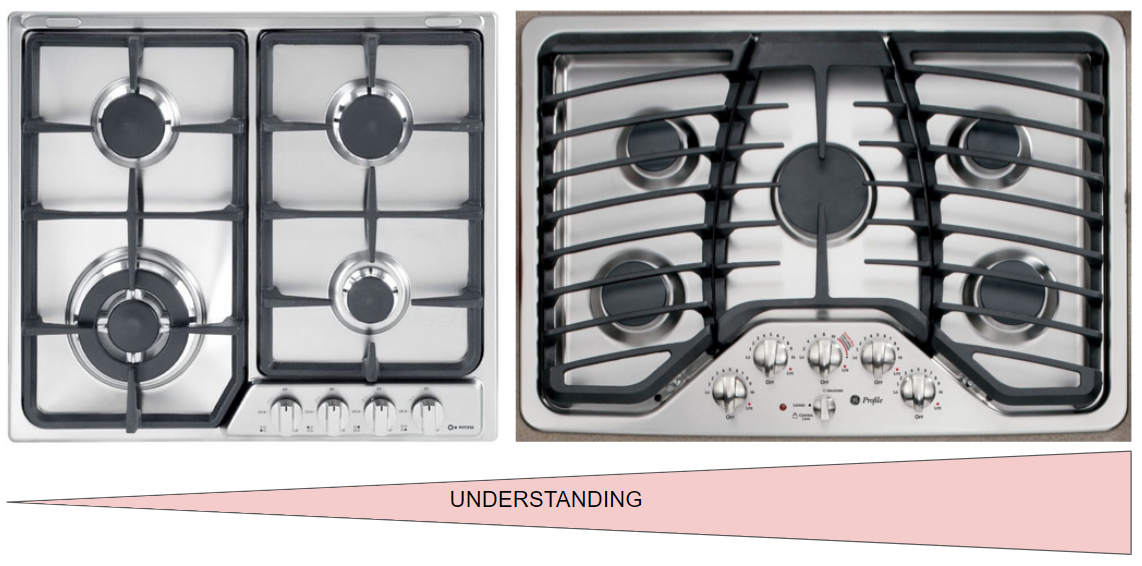
\includegraphics[width=\textwidth]{immagini/understanding.png}
	\caption{Understanding.}
\end{figure}


\section{Design of Useful Things}
\begin{flushleft}
	\textit{Quando le cose vanno bene, si dimenticano subito, quando vanno male non si dimenticano mai!}
\end{flushleft}

Questo fenomeno è noto a tutti, si tende a ricordare più facilmente le disavventure e i problemi che le belle esperienze, che spesso vengono percepite come ovvie e scontate. Questo accade perché ormai viviamo in una società in cui \textbf{le cose devono andare bene} per definizione. Quando qualcosa invece va storto, scattano tutta una serie di reazioni che portano la persona a provare sensazioni e emozioni spiacevoli, tipicamente frustrazione. 

Questo è un processo neurologico del tutto naturale che consente agli uomini di apprendere velocemente dalla propria esperienza andando ad etichettare le esperienze spiacevoli come più importanti rispetto a quelle positive. Dal punto di vista evolutivo, sbagliare vuol dire rischiare la vita mentre fare bene è solo l'ovvio cammino per la sopravvivenza.

Il design deve quindi preoccuparsi di come funzionano le cose, come vengono controllate e della natura delle interazioni che questi oggetti e sistemi abilitano con gli utenti. Gli oggetti, i software e i sistemi ben progettati danno vita ad esperienze d'uso piacevoli e rilassanti, quando un oggetto o un software sono mal progettati l'utente vive invece un'esperienza spiacevole caratterizzata da emozioni negative e dal desiderio di evitare in futuro di doversi imbattere nuovamente in un'esperienza simile.

Questo vuol dire che una cattiva esperienza utente induce l'utilizzatore non solo ad abbandonare l'utilizzo di un prodotto ma soprattutto porta la persona ad etichettare il prodotto e l'azienda produttrice come da evitare. 

Le \textbf{macchine} sono concepite, progettate e costruite da esseri umani ma sono ben diverse dai loro creatori. Le macchine sono sistemi logici, deterministici, prevedibili e con comportamenti basati su algoritmi fissi. L'uomo è invece aleatorio, versatile, variabile, volubile, e intuitivo. \textbf{Uno l'opposto dell'altro!}
Inoltre, le macchine non hanno esperienza (nell'accezione in cui la intendiamo tipicamente in neuroscienze). Per una macchina ogni azione, procedura e sequenza è nuova, si ricomincia sempre da zero. Non importa se l'utente ha già fatto quella procedura decine di volte, anche questa volta la macchina pretenderà che questa venga eseguita alla perfezione e seguendo tutti i passi richiesti.

Inoltre, le macchine al nostro confronto, sono \textbf{assai limitate}. Non possono fare qualsiasi cosa in maniera mediocre come noi ma sono concepite per fare poche cose (spesso solo una) in maniera eccellente. Anche in questo caso hanno un comportamento opposto rispetto a quello umano. Gli uomini sono in grado di fare tutto in maniera mediocre e qualche cosa in maniera eccellente e possono inoltre, con l'esperienza, cambiare le attività su cui eccellono. Le macchine nascono in un modo e muoiono invariate.

Le macchine seguono, di solito, \textbf{regole di comportamento rigide}, piuttosto complicate. Se si sbaglia nel seguirle, anche di poco, il sistema fallisce. La macchina esegue infatti quello che gli è stato richiesto, anche se questo è insensato e illogico. 

Questa analisi ci porta a concludere che \textit{le macchine obbligano le persone a smettere di comportarsi da umani inducendole a comportarsi da macchine.}

La tipica esperienza d'uso di un software è quella di un umano che impara le procedure imposte dal software, capisce come questo funziona ed è stato progettato e inizia così a ragionare come lui. L'umano asseconda la macchina per poter ottenere un risultato e procedere nell'esecuzione dell'attività senza intoppi.

\begin{flushleft}
	\textit{We have to humanize machines instead of dehumanizing humans} (David Hanson, Padre del robot Sophia della Hanson Robotics.)
\end{flushleft}

Questo condizione di schiavitù umana è dovuta al fatto che spesso le regole di funzionamento della macchina sono note solo alla macchina stessa e ai suoi progettisti. 

Come detto, quando non si eseguono queste regole segrete e bizzarre, la macchina fa la \textbf{cosa sbagliata} e la colpa è tipicamente accollata all'utente incapace. Quando questo accade con oggetti comuni, di uso domestico o personale, il risultato è la frustrazione dell'utente e il fallimento del prodotto. Quando invece questo fenomeno accade in contesti industriali e commerciali, le conseguenze possono essere incidenti mortali e importanti conseguenze economiche.

È tempo di \textbf{ribaltare la prospettiva}. 

\begin{flushleft}
	\textbf{Quando le cose vanno male la colpa non è mai dell'utente ma è sempre della macchina e quindi del progettista.}
\end{flushleft}

Questa prospettiva, apparentemente estrema, è in realtà il punto di partenza fondamentale per la progettazione di prodotti, sistemi e servizi usabili e quindi di successo. 

Le ragioni della complessità dell'interazione uomo-macchina sono numerose. Spesso però, la maggior causa del ``cattivo design'' è dovuta alla formazione dei tecnici e dei progettisti. Per molti anni si è focalizzato tutto il bagaglio formativo dei tecnici su tematiche tecnologiche ignorando gli aspetti legati alla psicologia umana e alle dinamiche di mercato.

La maggior parte dei problemi di design deriva quindi dalla totale incomprensione dei principi del design necessari per portare alla realizzazione di un prodotto capace di abilitare una positiva esperienza di interazione uomo-macchina.

Gli ingegneri, gli informatici sono eccellenti sul piano tecnico ma spesso sono molto limitati nella comprensione delle persone e della socialità.
I tecnici pensano: \textit{``Siamo uomini anche noi, quindi siamo in grado di capire i nostri simili e di progettare per loro.''}

Sbagliato! I tecnici falliscono perché partono da un'assunzione profondamente sbagliata e cioè che la spiegazione logica del funzionamento di un sistema sia sufficiente per consentire a chiunque di utilizzarlo. Purtroppo, come già detto, la logica e le persone non vanno molto d'accordo!

\begin{flushleft}
\textit{``Basterebbe che leggessero le istruzioni e tutto andrebbe bene!''}
\end{flushleft}


Gli ingegneri sono formati per utilizzare quotidianamente il pensiero logico e computazionale, di conseguenza finiscono per credere che quello sia il modo comune di ragionare. 


È quindi fondamentale accettare che il comportamento umano è illogico e non può essere modificato (per fortuna). 
\begin{flushleft}
\textbf{Bisogna progettare per come le persone sono e non per come vorremmo che fossero!}
\\
\textit{``we were designing things for people, so we needed to  understand both technology and people. But that’s a difficult step for many engineers: machines are so logical, so orderly. \\
If we didn’t have people, everything would work so much better. \\
Yup, that’s how I used to think.'' (Donald Norman)}
\end{flushleft}

\section{L'incidente di Three Mile Island }
Da: \url{https://it.wikipedia.org/wiki/Incidente_di_Three_Mile_Island}\\

L'incidente di Three Mile Island fu una parziale fusione del nocciolo avvenuto nella centrale nucleare sull'omonima isola, nella Contea di Dauphin, in Pennsylvania, il 28 marzo del 1979. Fu il più grave incidente nucleare avvenuto negli Stati Uniti d'America, e ha portato al rilascio di piccole quantità di gas radioattivi e di iodio radioattivo nell'ambiente.


L'incidente avvenne esattamente alle ore 4:00 di mercoledì 28 marzo 1979, quando il reattore era ad un regime di potenza del $97\%$. L'incidente ebbe inizio nel circuito di refrigerazione secondario, con il blocco della portata di alimentazione ai generatori di vapore. Questo blocco portò, nel circuito primario di raffreddamento del nocciolo, ad un considerevole aumento della pressione del refrigerante, causando prima l'apertura di una valvola PORV di rilascio posta sul pressurizzatore e poi lo ``SCRAM'' (arresto di emergenza del reattore mediante l'inserimento delle barre di controllo). 

A questo punto la valvola di rilascio non si richiuse e \emph{gli operatori non si resero conto del problema, anche perché non vi era nella strumentazione l'indicazione della reale posizione della valvola. La strumentazione era infatti legata all'alimentazione del motore della valvola e non alla reale posizione della valvola.}

Fu così che il circuito di raffreddamento primario si vuotò parzialmente e il calore residuo del nocciolo del reattore non poté essere smaltito. A causa di ciò il nocciolo radioattivo subì gravi danni. \emph{Gli operatori non poterono diagnosticare correttamente cosa avveniva e reagire in maniera adeguata. La strumentazione carente della sala controllo e l'addestramento inadeguato risultarono essere le cause principali dell'incidente.}

Durante l'incidente si ebbe una pericolosa fusione parziale del nocciolo e di conseguenza vennero riportati alcuni gravissimi danni; l'unità 2 fu chiusa ed è ancora oggi sotto monitoraggio, in attesa delle future azioni di smantellamento.

%I dispositivi complessi a causa della loro scarsa visibilità e della loro complessità richiedono di essere accompagnati da manuali d'istruzioni, ma questo è accettabile \textbf{solo} se il dispositivo è davvero complesso e dovrebbe essere del tutto \textbf{superfluo} per le cose \textbf{semplici}.

